\chapter{Position and Orientation}\label{ch:position_rotation}

As it has been shown before, once the threshold segmentation has been applied to our cropped image from the workspace, the picture will look something of this sort:

\begin{figure}[hb]
  \centering
  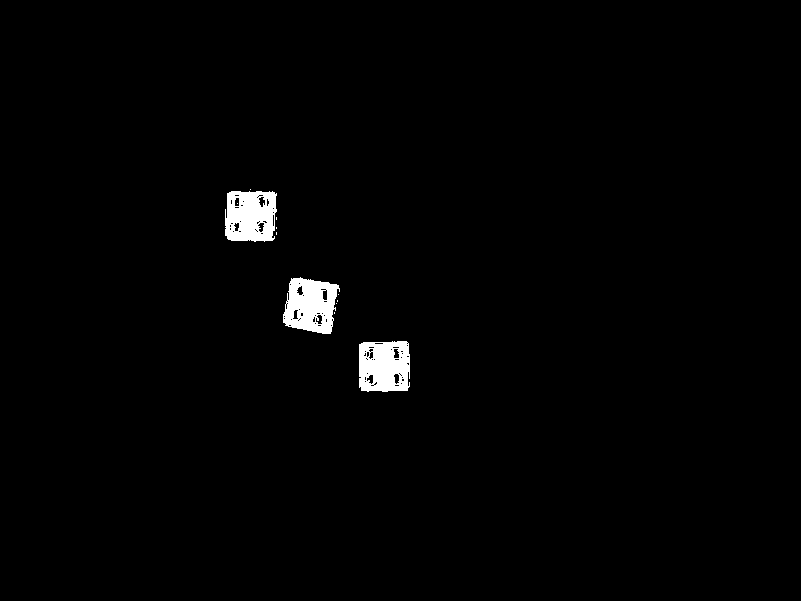
\includegraphics[scale=0.3]{figures/thresh_img.png}
  \caption[thresholded_image] {RGB Segmented Image}
\end{figure}

\subsection*{Position}
The goal of this project is to try to pick the bricks, creating Simpson characters with them. Therefore, it is imperative to have a precise position of every block in order to be able to give the correct coordinates to the gripper. This is the reason why the position becomes one of the most important steps in this project.

After computing the picture taken by the camera, the detection of the center involved the creation of areas that would be labeled. Hence, it was necessary to detect the edges of the bricks in order to find their squared shapes and, then, the square was filled, creating an homogeneous area.

Finally, \textit{Regionprops} function was used to detect the center of each white area (binary image). The detected center was the center of mass and not the geometrical one, however, the differences between them were very small because the area was homogeneously filled.


\subsection*{Orientation}
Besides the position, the measure of the required angle to turn the gripper is also essential to achieve the goal. Nevertheless, the coordinates of the center will be important to find the orientation of the bricks. 

First, four furthest points with respect to the center are necessary to find the coordinates of the corners. However, this search needs to be constrainted to ensure that the distance between each point is, at least, fifteen pixels, to avoid having more than one point in each corner.

Then, two of the previous corners are chosen in order to define one side of the square. The connection between these two corners and the center generates two different straight lines (from each corner to the center). Using the image with the edges of the desired block it was evaluated which points were below the generated lines. To finish this step, a linear regression was calculated and the parameters of the straight line were found.

\begin{figure}[h]
 
\begin{subfigure}{0.5\textwidth}
\captionsetup{justification=centering}

\includegraphics[scale=0.5]{figures/diag_square.png} 
\centering
\caption{Straight lines that connect the corners with the center of the brick}
\label{fig:subim1}
\end{subfigure}
\begin{subfigure}{0.5\textwidth}
\captionsetup{justification=centering}
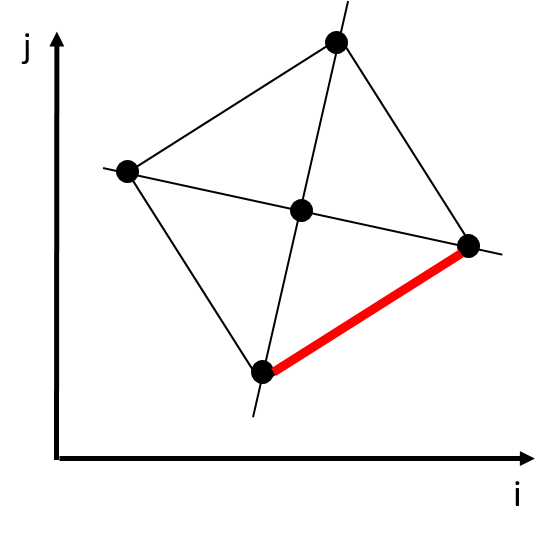
\includegraphics[scale=0.5]{figures/diag_square_side.png}
\centering
\caption{Side of the square used for calculating the slope}
\label{fig:subim2}
\end{subfigure}
 
\caption{Brick in the world frame}
\label{fig:image2}
\end{figure}

Finally, the slope was converted to an angle to obtain the orientation of the brick. However, if the angle was negative it was necessary to calculate the one associated with the perpendicular line in order to have the correct orientation.

\begin{figure}[h]
 
\begin{subfigure}{0.5\textwidth}
\captionsetup{justification=centering}
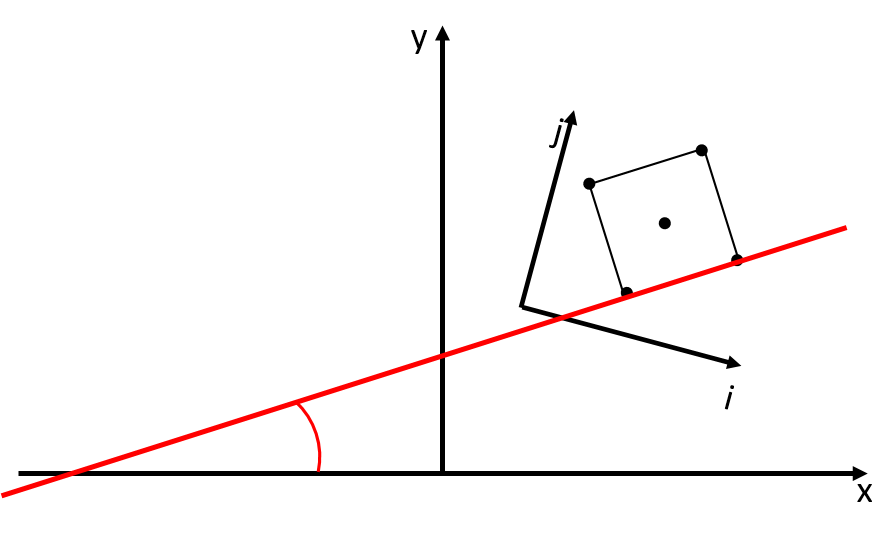
\includegraphics[scale=0.5]{figures/posit_slope.png}
\centering
\caption{Positive slope - it gives directly the orientation}
\label{fig:subim1}
\end{subfigure}
\begin{subfigure}{0.5\textwidth}
\captionsetup{justification=centering}
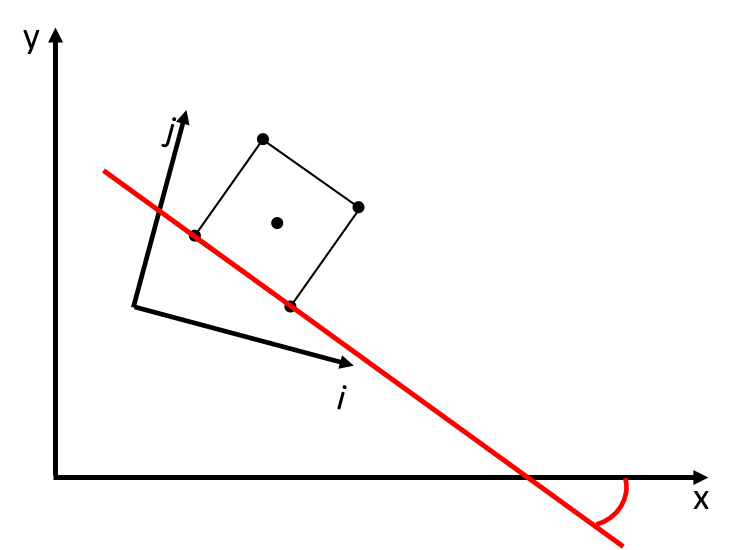
\includegraphics[scale=0.5]{figures/neg_slope.png}
\centering
\caption{Negative slope - it gives indirectly the orientation}
\label{fig:subim2}
\end{subfigure}
 
\caption{Orientation of the brick in the robot frame}
\label{fig:image2}
\end{figure}
